\documentclass{article}



\usepackage{fullpage}
\usepackage{nopageno}
\usepackage{amsmath}
\usepackage{amsfonts}
\usepackage{graphicx}
\usepackage{framed}
\usepackage{xcolor}

\definecolor{dark_red}{rgb}{0.5,0.0,0.0}
\definecolor{dark_green}{rgb}{0.0,0.5,0.0}
\definecolor{dark_blue}{rgb}{0.0,0.0,0.5}
\definecolor{blue}{rgb}{0.0,0.0,1.0}

\newcommand{\dr}[1]{\textcolor{dark_red}{#1}}
\newcommand{\dg}[1]{\textcolor{dark_green}{#1}}
\newcommand{\db}[1]{\textcolor{dark_blue}{#1}}
\newcommand{\blue}[1]{\textcolor{blue}{#1}}


\begin{document}




\section*{The square root of negative numbers}

Up until now, the square roots of negative numbers are treated as ``undefined". With the use of {\bf imaginary} or {\bf complex numbers}, the square roots of negative numbers can be defined.

To begin, the {\bf imaginary unit}, denoted by \(i\), is the square root of \(-1\):
\[i = \sqrt{-1}\]

For an arbitrary negative number \(x\), number \(x\) has the form \(x = -y\) where \(y\) is positive. The square root of \(x\) is defined by:
\[\sqrt{x} = \sqrt{-y} = i\sqrt{y}\]
It is easy to observe that:
\[(i\sqrt{y})^2 = i^2(\sqrt{y})^2 = (-1) \cdot y = -y = x\]
so \(i\sqrt{y}\) is indeed the square root of \(x\).

\textbf{Examples:}
\begin{itemize}
\item \(\sqrt{-2} = i\sqrt{2}\)
\item \(\sqrt{-4} = i\sqrt{4} = 2i\)
\item \(\sqrt{-5} = i\sqrt{5}\)
\item \(\sqrt{-9} = i\sqrt{9} = 3i\)
\end{itemize}




\section*{Complex numbers}

Any number \(z\) with the form \(z = yi\) where \(y\) is a real number (\(y \in \mathbb{R}\)) is referred to as a ``pure imaginary number".

Any number \(z\) with the form \(z = x + yi\) where \(x\) and \(y\) are real numbers (\(x \in \mathbb{R} \;\wedge\; y \in \mathbb{R}\)) is referred to as a {\bf complex number}. The set of complex numbers is denoted by \(\mathbb{C}\). It is important to note that the expression \(x + yi\) cannot be simplified any further. For every complex number \(z\), there is only one real value \(x\) and real value \(y\) such that \(z = x + yi\). Every unique choice of real numbers \(x\) and \(y\) corresponds to a unique complex number.  

For an arbitrary complex number \(z = x + yi\), \(x\) is the ``real component", while \(y\) is the ``imaginary component". The real and imaginary components are accessed by the functions:
\begin{itemize}
\item \(\text{Re}(z) = \text{Re}(x + yi) = x\)
\item \(\text{Im}(z) = \text{Im}(x + yi) = y\) 
\end{itemize}

While the set \(\mathbb{R}\) of {\bf real numbers} can be envisioned as a line, referred to as the real line, the set \(\mathbb{C}\) of {\bf complex numbers} can be envisioned as a \emph{plane}, referred to as the {\bf complex plane}. Given an arbitrary complex number \(z = x + yi\) where \(x\) and \(y\) are real numbers, the location of \(z\) on the complex plane is the point with Cartesian coordinates \((x,y)\). The real line is essentially the \(x\)-axis of the complex plane. The \(y\)-axis of the complex plane is referred to as the ``imaginary axis". The set of real numbers is a subset of the set of complex numbers, every real number also counts as a complex number: \(\mathbb{R} \subset \mathbb{C}\). \\
\begin{tabular}{cc}
\parbox{0.4\textwidth}{Example complex numbers include:
\begin{itemize}
\item \(-4\), \(-\pi\), \(-3\), \(-\sqrt{2}\), \(-2\), \(-1\), \(0\), \(1\), \(1.5\), \(2\), \(2.25\), \(3\), \(4\)
\item \(-4i\), \(-3i\), \(-2i\), \(-i\), \(i\), \(2i\), \(3i\), \(4i\)
\item \(1 + 2i\)
\item \(-3 + i\)
\item \(1 - i\)
\item \(-\frac{1}{\sqrt{2}} - \frac{i}{\sqrt{2}}\)
\item \(-2 - 2i\)
\item \(-2.5 + 2i\)
\item \(2.5 + 2.75i\)
\item \(2 - 3i\)
\item \(3 + 2i\)
\end{itemize}
all of which are marked on the complex plane on the right.
} & \parbox{0.6\textwidth}{
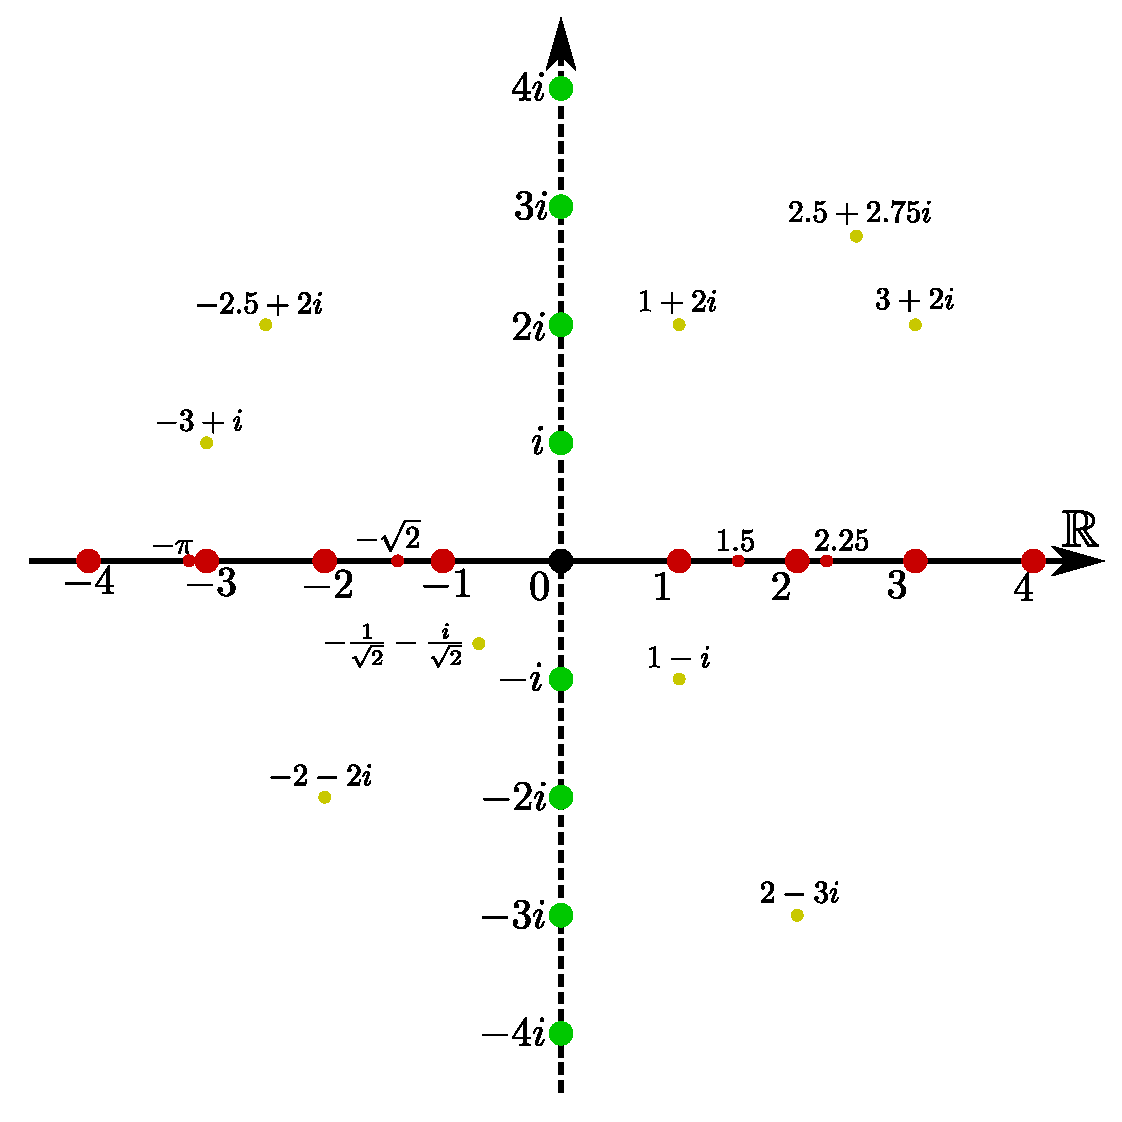
\includegraphics[width = 0.6\textwidth]{the_complex_plane_1}
}
\end{tabular}





\section*{Arithmetic using complex numbers}

When evaluating expressions involving complex numbers, the aim will always be an expression with the form 
\[x + yi\]
where \(x\) and \(y\) are real numbers. 

The basic properties of the arithmetic operators, addition, multiplication, subtraction, and division, are:    
\begin{itemize}
\item The operations of addition and multiplication are both commutative. For all numbers \(z\) and \(w\),
\begin{align*}
z + w = & w + z \\
zw = & wz
\end{align*} 
\item The operations of addition and multiplication are associative. For all numbers \(z\), \(w\), and \(u\),
\begin{align*}
(z + w) + u = & z + (w + u) \\
(zw)u = & z(wu)
\end{align*}
\item The addition of \(0\) to a number does not change the number:
\[z + 0 = z\]
\item The multiplication of \(1\) to a number does not change the number:
\[z \cdot 1 = z\]
\item The multiplication of \(0\) to a number results in \(0\):
\[z \cdot 0 = 0\]
\item Every number has a negative. For every number \(z\), there exists a negative \(-z\) that cancels out \(z\) via addition:
\[z + (-z) = 0\]
\item Every nonzero number has a reciprocal. For every number \(z\) where \(z \neq 0\), there exists a reciprocal \(z^{-1} = \frac{1}{z}\) that cancels out \(z\) via multiplication:
\[z \cdot z^{-1} = z \cdot \frac{1}{z} = 1\]
\item Multiplication distributes over addition. For all numbers \(z\), \(w\), and \(u\), 
\[z(w + u) = zw + zu\]
\item The operation of subtraction is simply:
\[z - w = z + (-w)\]
\item The operation of division is simply:
\[z/w = z \cdot w^{-1} = z \cdot (1/w)\]
\end{itemize}



\subsection*{The addition and subtraction of complex numbers}

The addition of two complex numbers, and the multiplication of a complex number by a real number, proceeds in a manner similar to {\bf vectors}:

\textbf{Addition:} \\
Given two vectors, \(\mathbf{v}_1 = \langle x_1, y_1 \rangle\) and \(\mathbf{v}_2 = \langle x_2, y_2 \rangle\), 
\[\mathbf{v}_1 + \mathbf{v}_2 = \langle x_1, y_1 \rangle + \langle x_2, y_2 \rangle = \langle x_1 + x_2, y_1 + y_2 \rangle\]
Given two complex numbers, \(z_1 = x_1 + y_1 i\) and \(z_2 = x_2 + y_2 i\), 
\[z_1 + z_2 = (x_1 + y_1 i) + (x_2 + y_2 i) = (x_1 + x_2) + (y_1 + y_2) i\]

\textbf{Negation:} \\
Given vector \(\mathbf{v} = \langle x, y \rangle\), 
\[-\mathbf{v} = -\langle x, y \rangle = \langle -x, -y \rangle\]
Given complex number \(z = x + y i\),
\[-z = -(x + y i) = -x - y i\]

\textbf{Multiplication by a real number:} \\
Given vector \(\mathbf{v} = \langle x, y \rangle\) and scalar \(k\),
\[k\mathbf{v} = k\langle x, y \rangle = \langle kx, ky \rangle\]
Given complex number \(z = x + y i\) and {\bf real} number \(k\),
\[kz = k(x + y i) = kx + ky i\]

\textbf{Examples:}
\begin{itemize}
%%%%%%%%%%%%
\item 
\[(5 - i) + (-7 + 3i) = (5 - 7) + (-1 + 3)i = -2 + 2i\]
%%%%%%%%%%%%
\item 
\[(3 - 6i) - (5 - 4i) = (3 - 6i) + (-5 + 4i) = (3 - 5) + (-6 + 4)i = -2 - 2i\]
%%%%%%%%%%%%
\item 
\[-3(6 - 7i) = (-3)(6) + (-3)(-7)i = -18 + 21i\]
%%%%%%%%%%%%
\item 
\[-(i + 5) - 4(5 - 2i) = (-5 - i) + (-20 + 8i) = -25 + 7i\]
\end{itemize}



\subsection*{The multiplication of complex numbers}

The multiplication of complex numbers is where the notion of complex numbers diverges from vectors.

Given two complex numbers \(z_1 = x_1 + y_1 i\) and \(z_2 = x_2 + y_2 i\)
\begin{align*}
z_1z_2 = & (x_1 + y_1 i)(x_2 + y_2 i) 
= x_1(x_2 + y_2 i) + y_1 i (x_2 + y_2 i)
= (x_1 x_2 + x_1 y_2 i) + (y_1 x_2 i + y_1 y_2 i^2) \\
& \text{the fact that } i^2 = -1 \text{ gives:} \\
= & (x_1 x_2 + x_1 y_2 i) + (y_1 x_2 i - y_1 y_2) 
= (x_1 x_2 - y_1 y_2) + (x_1 y_2 + y_1 x_2)i
\end{align*}

\textbf{Examples:}
\begin{itemize}
%%%%%%%%%%%%
\item 
\begin{align*}
(7 + 9i)(8 + 6i) = & ((7)(8) - (9)(6)) + ((7)(6) + (9)(8))i \\
= & (56 - 54) + (42 + 72)i 
= 2 + 114i
\end{align*}
%%%%%%%%%%%%
\item 
\begin{align*}
(-7 + 4i)(6 - 5i) = & ((-7)(6) - (4)(-5)) + ((-7)(-5) + (4)(6))i \\
= & (-42 + 20) + (35 + 24)i 
= -22 + 59i
\end{align*}
%%%%%%%%%%%%
\item 
\begin{align*}
(-7 - 2i)(-6 + 3i) = & ((-7)(-6) - (-2)(3)) + ((-7)(3) + (-2)(-6))i \\
= & (42 + 6) + (-21 + 12)i 
= 48 - 9i
\end{align*}
\end{itemize}



\subsection*{The division of complex numbers}

The division of a complex number \(z = x + y i\) by real number \(k\) is a trivial matter:
\begin{align*}
\frac{z}{k} = & \frac{x + y i}{k} 
= \frac{x}{k} + \frac{y}{k} i
\end{align*}

If the divisor (denominator) is complex, division is far less trivial. To begin, the concept of the {\bf complex conjugate} will be defined. 

Given a complex number \(z = x + yi\), the {\bf complex conjugate} (referred to simply as the conjugate) of \(z\) is denoted by \(\bar{z}\) or \(z^*\) and is defined by:
\[\bar{z} = z^* = x - y i\] 

Multiplying \(z = x + y i\) by its conjugate gives:
\[z z^* = (x + y i)(x - y i) = ((x)(x) - (y)(-y)) + ((x)(-y) + (y)(x))i = (x^2 + y^2) + (-xy + xy)i = x^2 + y^2\]
which is a {\bf real number}. Given a quotient involving complex numbers \(z_1 = x_1 + y_1 i\) and \(z_2 = x_2 + y_2 i\),
\[\frac{z_1}{z_2} = \frac{x_1 + y_1 i}{x_2 + y_2 i}\]
Multiplying the top and bottom of this fraction by the conjugate of \(z_2\) will yield the real number \(x_2^2 + y_2^2\) in the denominator: 
\begin{align*}
\frac{z_1}{z_2} = & \frac{x_1 + y_1 i}{x_2 + y_2 i}
= \frac{(x_1 + y_1 i)(x_2 - y_2 i)}{(x_2 + y_2 i)(x_2 - y_2 i)} 
= \frac{(x_1 + y_1 i)(x_2 - y_2 i)}{x_2^2 + y_2^2} 
\end{align*}
With the denominator now real, the complex arithmetic proceeds in a simple manner. 

\textbf{Examples:}
\begin{itemize}
%%%%%%%%%%%%
\item 
\begin{align*}
\frac{3 + 5i}{2 - i} 
= & \frac{(3 + 5i)(2 + i)}{(2 - i)(2 + i)} 
= \frac{(6 - 5) + (3 + 10)i}{4 + 1}
= \frac{1 + 13i}{5} 
= \frac{1}{5} + \frac{13}{5}i
\end{align*}
%%%%%%%%%%%%
\item 
\begin{align*}
\frac{29 - 2i}{3 - 2i} 
= & \frac{(29 - 2i)(3 + 2i)}{(3 - 2i)(3 + 2i)}  
= \frac{(87 + 4) + (58 - 6)i}{9 + 4} 
= \frac{91 + 52i}{13} 
= 7 + 4i
\end{align*}
%%%%%%%%%%%%
\item 
\begin{align*}
\frac{-40 + 4i}{-2 - 2i} 
= & \frac{(-40 + 4i)(-2 + 2i)}{(-2 - 2i)(-2 + 2i)}  
= \frac{(80 - 8) + (-80 - 8)i}{4 + 4} 
= \frac{72 - 88i}{8} 
= 9 - 11i
\end{align*}
%%%%%%%%%%%%
\item 
\begin{align*}
\frac{7 - 5i}{-2 + i} 
= & \frac{(7 - 5i)(-2 - i)}{(-2 + i)(-2 - i)} 
= \frac{(-14 - 5) + (-7 + 10)i}{4 + 1} 
= \frac{-19 + 3i}{5}  
= -\frac{19}{5} + \frac{3}{5}i
\end{align*}
%%%%%%%%%%%%
\item 
\begin{align*}
\frac{1 + 13i}{3 - i} 
= & \frac{(1 + 13i)(3 + i)}{(3 - i)(3 + i)} 
= \frac{(3 - 13) + (1 + 39)i}{9 + 1}
= \frac{-10 + 40i}{10} 
= -1 + 4i  
\end{align*}
%%%%%%%%%%%%
\item 
\begin{align*}
\frac{-2 - 14i}{-3 + 4i} 
= & \frac{(-2 - 14i)(-3 - 4i)}{(-3 + 4i)(-3 - 4i)} 
= \frac{(6 - 56) + (8 + 42)i}{9 + 16}
= \frac{-50 + 50i}{25} 
= -2 + 2i 
\end{align*}
\end{itemize}


\subsection*{Absolute values of complex numbers}

The ``absolute value" or ``magnitude" of a complex number \(z = x + yi\) is the ``distance" that \(z\) is from \(0\) on the complex plane. This is how far the Cartesian coordinate \((x, y)\) is from the origin, and is the length of the vector \(\langle x, y \rangle\). The vector \(\langle x, y \rangle\) has the length \(\|\langle x, y \rangle\| = \sqrt{x^2 + y^2}\). Therefore the absolute value of \(z\), denoted by \(|z|\) or \(\|z\|\), is 
\[|z| = |x + yi| = \sqrt{x^2 + y^2}\]
Note that if \(z\) is a real number, where \(y = 0\), then \(|z| = \sqrt{x^2 + y^2} = \sqrt{x^2 + 0^2} = \sqrt{x^2} = |x|\), which means that the definition of the absolute value for complex numbers is consistent with the absolute value for real numbers. The absolute value does not have multiple meanings for real numbers.

\textbf{Examples:}
\begin{itemize}
%%%%%%%%%%%%
\item 
\[\big| -3 + 4i \big| = \sqrt{(-3)^2 + 4^2} = \sqrt{9 + 16} = \sqrt{25} = 5\]  
%%%%%%%%%%%%
\item 
\[\big| i - 2 \big| = \sqrt{(-2)^2 + 1^2} = \sqrt{4 + 1} = \sqrt{5}\]
%%%%%%%%%%%%
\item 
\[\big| (-7i + 11) - 3(6 - 2i) \big| = \big| (11 - 7i) + (-18 + 6i) \big| = \big| -7 - i \big| = \sqrt{(-7)^2 + (-1)^2} = \sqrt{49 + 1} = \sqrt{50} = 5\sqrt{2}\]
\end{itemize}

Given an arbitrary complex number \(z\), it should also be noted that since \(z z^* = x^2 + y^2\), the product of \(z\) with its complex conjugate is the square of the absolute value:
\[|z|^2 = z z^*\]





\section*{Quadratic equations and complex numbers}

Consider an arbitrary quadratic equation:

\[ax^2 + bx + c = 0\] 

where \(a\), \(b\), and \(c\) are fixed constants. The constants \(a\), \(b\), and \(c\) will always be {\bf real} valued. The solutions are given by the quadratic equation:

\[x = \frac{-b \pm \sqrt{b^2 - 4ac}}{2a}\]

The discriminant \(\Delta = b^2 - 4ac\) determines the number and types of solutions:
\begin{itemize}
\item \(\Delta > 0\) means that there are two {\bf real} valued solutions. 
\item \(\Delta = 0\) means that there is one {\bf real} valued solution. 
\item \(\Delta < 0\) means that there are two {\bf complex} valued solutions, with nonzero imaginary components.
\end{itemize}
Previously, when \(\Delta < 0\), there were no solutions when confined to the set real numbers. Now however, there are two complex solutions.


\textbf{Examples:}
\begin{itemize}
%%%%%%%%%%%%
\item Consider the equation: 
\[3x^2 - 3x + 1 = 0\]
\(a = 3\), \(b = -3\), and \(c = 1\) so the quadratic formula gives:
\begin{align*}
x = & \frac{-b \pm \sqrt{b^2 - 4ac}}{2a} 
= \frac{3 \pm \sqrt{9 - 12}}{6} 
= \frac{3 \pm \sqrt{-3}}{6} 
= \frac{3 \pm i\sqrt{3}}{6} \\
= & \frac{1}{2} \pm \frac{\sqrt{3}}{6} i
\end{align*}
Therefore
\[x = \frac{1}{2} \pm \frac{\sqrt{3}}{6} i\]
and there are 2 {\bf complex} valued solutions. These quantities cannot be evaluated further without the use of approximations. We will verify our solutions by substituting them back into the original equation:
\begin{align*}
3x^2 - 3x + 1 
= & 3\left(\frac{1}{2} \pm \frac{\sqrt{3}}{6} i\right)^2 - 3\left(\frac{1}{2} \pm \frac{\sqrt{3}}{6} i\right) + 1 \\
= & 3\left(\frac{1}{4} \pm \frac{\sqrt{3}}{6}i - \frac{3}{36}\right) + \left(-\frac{3}{2} \mp \frac{\sqrt{3}}{2} i\right) + 1 \\
= & \left(\frac{3}{4} \pm \frac{\sqrt{3}}{2}i - \frac{1}{4}\right) - \frac{1}{2} \mp \frac{\sqrt{3}}{2} i \\
= & 0 \pm \frac{\sqrt{3}}{2}i \mp \frac{\sqrt{3}}{2} i \\
= & 0
\end{align*}
Therefore the solutions satisfy the original equation.
%%%%%%%%%%%%
\item Consider the equation: 
\[x^2 - 3x + 4 = 0\]
\(a = 1\), \(b = -3\), and \(c = 4\) so the quadratic formula gives:
\begin{align*}
x = & \frac{-b \pm \sqrt{b^2 - 4ac}}{2a} 
= \frac{3 \pm \sqrt{9 - 16}}{2} 
= \frac{3 \pm \sqrt{-7}}{2} 
= \frac{3 \pm i\sqrt{7}}{2} 
\end{align*}
Therefore:
\[x = \frac{3 \pm i\sqrt{7}}{2}\]
and there are 2 {\bf complex} valued solutions. These quantities cannot be evaluated further without the use of approximations. We will verify our solutions by substituting them back into the original equation:
\begin{align*}
x^2 - 3x + 4
= & \left(\frac{3 \pm i\sqrt{7}}{2}\right)^2 - 3\left(\frac{3 \pm i\sqrt{7}}{2}\right) + 4 \\
= & \frac{9 \pm 6\sqrt{7} \cdot i - 7}{4} + \frac{-9 \mp 3\sqrt{7} \cdot i}{2} + 4 \\
= & \frac{(2 \pm 6\sqrt{7} \cdot i) + (-18 \mp 6\sqrt{7} \cdot i) + 16}{4} \\
= & \frac{0 \pm 6\sqrt{7} \cdot i \mp 6\sqrt{7} \cdot i}{4} \\
= & 0
\end{align*}
Therefore the solutions satisfy the original equation.
%%%%%%%%%%%%
\item Consider the equation: 
\[x^2 - 3x + 1 = 0\]
\(a = 1\), \(b = -3\), and \(c = 1\) so the quadratic formula gives:
\begin{align*}
x = & \frac{-b \pm \sqrt{b^2 - 4ac}}{2a} 
= \frac{3 \pm \sqrt{9 - 4}}{2} 
= \frac{3 \pm \sqrt{5}}{2}
\end{align*}
Therefore:
\[x = \frac{3 \pm \sqrt{5}}{2}\]
and there are 2 {\bf real} valued solutions. These quantities cannot be evaluated further without the use of approximations. We will verify our solutions by substituting them back into the original equation:
\begin{align*}
x^2 - 3x + 1 
= & \left(\frac{3 \pm \sqrt{5}}{2}\right)^2 - 3\left(\frac{3 \pm \sqrt{5}}{2}\right) + 1 \\
= & \frac{9 \pm 6\sqrt{5} + 5}{4} + \frac{-9 \mp 3\sqrt{5}}{2} + 1 \\
= & \frac{(14 \pm 6\sqrt{5}) + (-18 \mp 6\sqrt{5}) + 4}{4} \\
= & \frac{0 \pm 6\sqrt{5} \mp 6\sqrt{5}}{4} \\
= & 0 
\end{align*}
Therefore the solutions satisfy the original equation.
%%%%%%%%%%%%
\item Consider the equation: 
\[5x^2 - 9x + 3 = 0\]
\(a = 5\), \(b = -9\), and \(c = 3\) so the quadratic formula gives:
\begin{align*}
x = & \frac{-b \pm \sqrt{b^2 - 4ac}}{2a} 
= \frac{9 \pm \sqrt{81 - 60}}{10} 
= \frac{9 \pm \sqrt{21}}{10}
\end{align*}
Therefore:
\[x = \frac{9 \pm \sqrt{21}}{10}\]
and there are 2 {\bf real} valued solutions. These quantities cannot be evaluated further without the use of approximations. We will verify our solutions by substituting them back into the original equation:
\begin{align*}
5x^2 - 9x + 3 
= & 5\left(\frac{9 \pm \sqrt{21}}{10}\right)^2 - 9\left(\frac{9 \pm \sqrt{21}}{10}\right) + 3 \\
= & 5\left(\frac{81 \pm 18\sqrt{21} + 21}{100}\right) + \frac{-81 \mp 9\sqrt{21}}{10} + 3 \\
= & \frac{102 \pm 18\sqrt{21}}{20} + \frac{-81 \mp 9\sqrt{21}}{10} + 3 \\
= & \frac{(102 \pm 18\sqrt{21}) + (-162 \mp 18\sqrt{21}) + 60}{20} \\
= & \frac{0 \pm 18\sqrt{21} \mp 18\sqrt{21}}{20} \\
= & 0
\end{align*}
Therefore the solutions satisfy the original equation.
%%%%%%%%%%%%
\item Consider the equation: 
\[-9x^2 + 12x + 1 = 0\]
\(a = -9\), \(b = 12\), and \(c = 1\) so the quadratic formula gives:
\begin{align*}
x = & \frac{-b \pm \sqrt{b^2 - 4ac}}{2a} 
= \frac{-12 \pm \sqrt{144 + 36}}{-18} 
= \frac{-12 \pm \sqrt{180}}{-18} 
= \frac{-12 \pm 6\sqrt{5}}{-18} \\
= & \frac{2 \mp \sqrt{5}}{3}
\end{align*}
Therefore:
\[x = \frac{2 \mp \sqrt{5}}{3}\]
and there are 2 {\bf real} valued solutions. These quantities cannot be evaluated further without the use of approximations. We will verify our solutions by substituting them back into the original equation:
\begin{align*}
-9x^2 + 12x + 1 
= & -9\left(\frac{2 \mp \sqrt{5}}{3}\right)^2 + 12\left(\frac{2 \mp \sqrt{5}}{3}\right) + 1 \\
= & -9\left(\frac{4 \mp 4\sqrt{5} + 5}{9}\right) + (8 \mp 4\sqrt{5}) + 1 \\
= & (-9 \pm 4\sqrt{5}) + (9 \mp 4\sqrt{5}) \\
= & 0 \pm 4\sqrt{5} \mp 4\sqrt{5} \\
= & 0
\end{align*}
Therefore the solutions satisfy the original equation.
%%%%%%%%%%%%
\item Consider the equation: 
\[x^2 - 6x + 10 = 0\]
\(a = 1\), \(b = -6\), and \(c = 10\) so the quadratic formula gives:
\begin{align*}
x = & \frac{-b \pm \sqrt{b^2 - 4ac}}{2a} 
= \frac{6 \pm \sqrt{36 - 40}}{2} 
= \frac{6 \pm \sqrt{-4}}{2} 
= \frac{6 \pm 2i}{2} \\
= & 3 \pm i
\end{align*}
Therefore:
\[x = 3 \pm i\]
and there are 2 {\bf complex} valued solutions. These quantities cannot be evaluated further without the use of approximations. We will verify our solutions by substituting them back into the original equation:
\begin{align*}
x^2 - 6x + 10
= & (3 \pm i)^2 - 6(3 \pm i) + 10 \\
= & (9 \pm 6i - 1) + (-18 \mp 6i) + 10 \\
= & 0 \pm 6i \mp 6i \\
= & 0
\end{align*}
Therefore the solutions satisfy the original equation.
\end{itemize}






\end{document}













